\documentclass{article}

\usepackage[utf8]{inputenc}
\usepackage[spanish]{babel}
\usepackage{listingsutf8}
\usepackage{xcolor}
\usepackage{pdfpages}
\usepackage{geometry}
% to install algorithm2e pckg: sudo apt-get install texlive-science
\usepackage[ruled, vlined, nofillcomment]{algorithm2e}
\usepackage{float}
\usepackage{hyperref}
\usepackage{amsmath}
\usepackage{framed}
\usepackage{enumitem}
\usepackage{svg}

\geometry{
    a4paper,
    margin=1.2in
}

% Some settings for coding style
\lstset{
    basicstyle=\linespread{0.9}\ttfamily\footnotesize,
    frame=single,
    frameround=tttt,
    numbers=left,
    numberstyle=\tiny,
    linewidth=14cm,
    literate=
      {á}{{\'a}}1 {é}{{\'e}}1 {í}{{\'i}}1 {ó}{{\'o}}1 {ú}{{\'u}}1
      {Á}{{\'A}}1 {É}{{\'E}}1 {Í}{{\'I}}1 {Ó}{{\'O}}1 {Ú}{{\'U}}1
      {à}{{\`a}}1 {è}{{\`e}}1 {ì}{{\`i}}1 {ò}{{\`o}}1 {ù}{{\`u}}1
      {À}{{\`A}}1 {È}{{\'E}}1 {Ì}{{\`I}}1 {Ò}{{\`O}}1 {Ù}{{\`U}}1
      {ä}{{\"a}}1 {ë}{{\"e}}1 {ï}{{\"i}}1 {ö}{{\"o}}1 {ü}{{\"u}}1
      {Ä}{{\"A}}1 {Ë}{{\"E}}1 {Ï}{{\"I}}1 {Ö}{{\"O}}1 {Ü}{{\"U}}1
      {â}{{\^a}}1 {ê}{{\^e}}1 {î}{{\^i}}1 {ô}{{\^o}}1 {û}{{\^u}}1
      {Â}{{\^A}}1 {Ê}{{\^E}}1 {Î}{{\^I}}1 {Ô}{{\^O}}1 {Û}{{\^U}}1
      {œ}{{\oe}}1 {Œ}{{\OE}}1 {æ}{{\ae}}1 {Æ}{{\AE}}1 {ß}{{\ss}}1
      {ű}{{\H{u}}}1 {Ű}{{\H{U}}}1 {ő}{{\H{o}}}1 {Ő}{{\H{O}}}1
      {ç}{{\c c}}1 {Ç}{{\c C}}1 {ø}{{\o}}1 {å}{{\r a}}1 {Å}{{\r A}}1
      {€}{{\euro}}1 {£}{{\pounds}}1 {«}{{\guillemotleft}}1
      {»}{{\guillemotright}}1 {ñ}{{\~n}}1 {Ñ}{{\~N}}1 {¿}{{?`}}1
}

\title{66.26 - Arquitecturas Paralelas\\Trabajo final}

\author{
    \\\\\\\\
%     \Large{Group name}\\
    Arturi, Augusto(\texttt{\#97498})\\\texttt{turitoh@gmail.com}\\
    \\
    Rozanec, Matias (\texttt{\#97404})\\\texttt{rozanecm@gmail.com}\\
%    \\
%    surname2, name2 (\texttt{\#padron})\\\texttt{mail@example.com}\\
    \\\\\\\\\\\\\\
}

\date{Diciembre 2018}

\begin{document}
\maketitle
\begin{figure}[!htp]
    \centering
    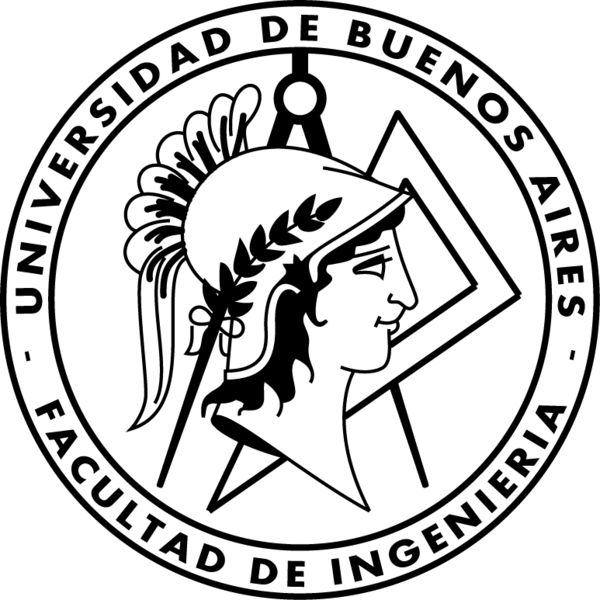
\includegraphics[scale=1]{../res/fiuba_logo.png} 
\end{figure}
\begin{center}\normalsize{Facultad de Ingeniería, Universidad de Buenos Aires}\end{center}
\newpage

\tableofcontents
\newpage

% *** CONSIGNA ***
% \part{Consigna}
% \includepdf[pages=-]{consigna.pdf}

% *** RESOLUCION ***

\section{Introducción}

La Dinámica de Fluidos (CFD por sus siglas en inglés) se usa para simular el flujo de fluidos en aplicaciones industriales. A medida que los simuladores se vuelven más complejos, el poder de cálculo que se requiere aumenta significativamente. En casos en que el tiempo de cómputo puede llevar días o meses, aún cambios relativamente pequeños en la eficiencia de cálculo pueden representar grandes mejoras en el cómputo.

El código usado para correr las simulaciones es OpenFOAM, un paquete CFD open source. Este software es diseñado para correr en paralelo, pudiendo ser configurado para correr efectivamente en cualquier cantidad de cores distribuidos a lo largo de cualquier número de computadoras presentes en una misma red. Idealmente los casos que se puedan correr en paralelo serán divididos en partes iguales distribuidas en cuantas unidades de procesamiento haya disponibles. Si cada proceso es capaz de correr independientemente, entonces el speedup será (en teoría) linealmente proporcional al incremento del hardware de cómputo. 

Debido a la naturaleza de los cálculos de CFD, OpenFOAM requiere un nivel significativo de comunicaciones inter-proceso para asegurar resultados consistentes en el dominio del caso. Esto significa que aunque el software sea en teoría infinitamente paralelizable, cada proceso adicional agrega costo comunicacional que reduce el speedup. Adicionalmente, a medida que el tamaño del hardware crece, varios cuellos de botella del sistema, como la latencia de la red, pueden obstaculizar posibles mejoras y llegar a un límite en que ya no convenga agregar más hardware. Estas limitaciones que se encuentran en la práctica hay que encararlas con especial cuidado, ya que es lo que define el nivel del grano con que se va a trabajar en la paralelización: de tener un problema no demasiado grande, es probable que recurrir a un grano fino, o sea, subdividir el problema en partes muy pequeñas, no termine rindiendo tan bien como se esperaba debido a que el costo comunicacional probablemente supere la ventaja de paralelizar el problema, quedando esta última muy disminuida o incluso anulada. 

En el presente trabajo se realizaron varias mediciones que permiten apreciar el desempeño en varios escenarios.

\newpage
\section{Herramientas}
\subsection{Hardware}
\begin{description}[align=right]
    \item [PC1] Intel Core i5-7200U 2.5 GHz with Turbo Boost up to 3.1 Ghz\\
        2 núcleos, 4 subprocesos.\\
        2 canales de memoria\\
        6 GB DDR4 memoria RAM  2400 MHz
    \item [PC2] AMD Ryzen 5 2400G 3.6GHz\\
        4 nucleos, 8 subprocesos.\\
        2 canales de memoria\\
        16 GB DDR4 memoria RAM 2400 MHz
    \item [PC3] Intel Core i5-5200U CPU @ 2.20GHz 3M Cache, up to 2.70 GHz\\
        2 nucleos, 4 subprocesos.\\
        2 canales de memoria\\
        8 GB DDR4 memoria RAM 2400 MHz
\end{description}
\subsection{Software}
\subsubsection{Software de resolución numérica}
El software utilizado para la resolución de problemas numéricos es OpenFOAM, un software de código abierto desarrollado por OpenCFD Ltd. desde 2004. Éste es utilizado en muchas áreas de ciencia e ingeniería, tanto en ámbitos comerciales como educativos. OpenFOAM presenta una amplia gama de características que le permite resolver una amplísima gama de problemas de fluidos, incluyendo pero no limitándose a reacciones químicas, turbulencias, transferencia de calor, acústica, mecánica de sólidos y electromagnetismo entre otros. 

\subsubsection{Software de paralelización}
Para poder correr el solver en paralelo, se hace uso de mpirun (Open MPI) versión 1.10.2. 

\subsubsection{Software de medición de tiempo}
Debido a que el programa puede ser operado desde una terminal, las mediciones de las corridas se han podido realizar directamente mediante el comando time, obteniendo las siguientes mediciones: 
\begin{description}[align=left]
    \item [Real:] mide el tiempo desde que arrancó a correr el programa hasta que terminó. Este tiempo incluye los time slices que el procesador está ocupado con otros procesos no relacionados con el programa de interés. Sin embargo, como esto siempre sucede en un sistema real\footnote{ Un sistema operativo siempre distribuye el tiempo de procesador de la mejor forma posible, y si bien puede haber tareas más importantes que otras, siempre habrá algunos procesos que requerirán algún tiempo de CPU, aunque el mismo sea mínimo, por lo que habrá ciclos de clock dedicados a tareas varias distintas a la medida.}, al haber hecho las mediciones corriendo solamente el software de interés sin otros procesos importantes de fondo, se puede considerar esta medición como buena.
    \item [User:] mide tiempo en que la CPU está ocupada en modo usuario. Notar que este tiempo en teoría no podría ser mayor al tiempo Real, sin embargo esto no es cierto si se corre un proceso en varios procesadores: en tal caso, User indica el total de tiempo contemplando a todas las CPUs, por lo que se esperan tiempos mayores al Real.
    \item [Sys:] mide tiempo en que la CPU está ocupada en modo kernel.
\end{description}

\newpage
\section{Análisis preliminar}
\subsection{Hardware}
Hay una variedad de factores de hardware que pueden afectar la eficiencia en el cálculo de CFD.
\begin{description}
    \item [Velocidad de CPU/RAM:] se listan la velocidad de cores y velocidad de RAM de las PC utilizadas para las simulaciones, notando que OpenFoam es una aplicación de alto consumo de memoria, por ende se espera una mejor perfomance en aquellas RAM con mayor frecuencia de clock.
    \item [Canales de memoria RAM:] tanto la velocidad de la memoria RAM como el número de canales entre la CPU y la memoria compartida puede afectar la velocidad de una simulación CFD. Dado que los procesadores que se utilizan tienen 2 canales de memoria, cuando la cantidad de cores activos sea mayor a 2 y el canal de memoria esté saturado dado el límite de ancho de banda, algunos cores quedarán en idle hasta que se transfiera toda la información a memoria, este proceso puede enlentecer la simulación.
    \item [Turbo boost:] la capacidad de overclockear el procesador con el fin de aumentar su frecuencia, es una  opción que puede maximizar la performance a un alto riesgo de dañar el CPU. Otra forma es utilizar el turbo, capacidad que solo tienen los chips Intel, que es una función designada a operar solo cuando unos pocos cores del CPU están siendo utilizados y el calor excedente producido por la disipacion de energia puede ser distribuido a lo largo del mecanismo de cooling del chip. Teóricamente, si todos los cores están siendo utilizados simultáneamente, el turbo boost no se activa.
    \item [Hyper-threading:] esta característica le permite a cada núcleo del CPU presentarse al sistema operativo como si fuesen dos, de los que uno será real y el otro virtual. Luego el SO puede asignar trabajos a los cores virtuales y asignarles trabajo cuando los cores reales están en idle (como por ejemplo esperando una lectura/escritura en memoria), de esta forma se maximiza la utilización del CPU. Sin embargo, OpenFoam es generalmente una aplicacion de uso intensivo de memoria: en raros casos durante una simulación CFD, la utilización de la CPU baja del 100\%, por lo tanto incrementar el número de procesos incrementará la comunicación, generando más overhead, en conclusión a priori se podría decir que este factor afectaría a cualquier beneficio de la utilización de cores virtuales, se espera demostrarlo en el presente trabajo.
\end{description}
\subsection{Software}
\begin{description}
    \item [Binding and distribution:] el método por el cual los procesos que se ejecutan son alocados y limitados en los cores, tienen un impacto muy significativo en la velocidad del paralelismo, la proximidad de los procesos en la arquitectura de hardware afecta la velocidad y eficiencia del proceso de intercomunicación.
        En una computadora de escritorio la asignación de los procesos es provista por el scheduler del sistema operativo en uso, el cual hará lo necesario para balancear la carga y ejecutar los procesos de la mejor manera posible, a su vez esta tarea podría implicar mover procesos entre distintos cores, siempre con la intención de mejorar la performance. Las aplicaciones CFD asignan los datos discretos a cada proceso en paralelo que es guardado en la memoria de cada núcleo, si por alguna razón el SO decide mover el proceso a un core el cual en memoria no tiene los datos necesarios, la información debe ser reescrita en la memoria de este para que el trabajo pueda continuar; esto produce un efecto perjudicial a la performance.\\
        
        Sin embargo, OpenMPI provee algunas primitivas para que en su ejecución se eviten este tipo de reasignaciones antes de que el trabajo sea terminado mediante el binding de un proceso a un core particular.
    \item [Case size and decomposition:] cuando una simulación es preparada para correr en paralelo, el dominio total es repartido en piezas del mismo tamaño, las cuales se asignan acorde a la cantidad de cores disponibles. Así como el número de procesos incrementa, cada pieza se torna más pequeña y el cálculo se completa más rápidamente, pero tal como se comentó anteriormente, incrementar el paralelismo implica incrementar las intercomunicaciones en orden de mantener el resultado esperado consistente. Como resultado, el número de procesos a paralelizar alcanza un máximo práctico, donde el speedup no se puede mejorar dado el aumento de tiempo en comunicación. Para un caso dado, este punto máximo es importante de encontrar para asegurar que los recursos computacionales no son desperdiciados en vano.\\
        
        El método por el cual es descompuesto el dominio afecta el tamaño y la forma de cada pieza de este, así como también el orden en el que estas son numeradas, lo cual  afecta a las posiciones relativas dentro del dominio (distancia dentro del procesador).\\

        OpenFoam provee de 4 métodos de descomposición:
        \begin{description}
            \item [Simple:] la descomposición es geométrica en la cual el dominio se divide en partes a partir de la dirección en los ejes x,y,z. Esta forma se suele utilizar en problemas en los cuales la naturaleza del problema es simétrico.
            \item [Jerárquica:] es igual a la simple con la salvedad de que el usuario puede especificar el orden en el cual quiere se divida por eje, es decir, primero por el eje Y, luego X y finalmente Z por ejemplo.
            \item [Scotch:] esta descomposición es un poco más interesante ya que no divide geométricamente por igual, por lo cual suele ser la más apropiada en problemas de la vida real. Esta forma intenta minimizar las comunicaciones entre los procesadores haciendo que los límites entre estos sean los menores posibles; más adelante se lo explicará con un ejemplo práctico. A su vez se pueden asignar pesos a los trabajos por procesador, característica útil en caso de tener a disposición chips de distinta frecuencia para realizar la simulación.
            \item [Manual:] el usuario especifica directamente la locación del área que se le asigna a cada procesador. Sin embargo, en un ejemplo en el cual se tienen que asignar una alta cantidad (millones) de celdas el proceso puede ser tedioso o impráctico.
        \end{description}

\end{description}

\newpage
\section{Casos de estudio}
El software OpenFOAM incluye en su instalación una enorme cantidad de tutoriales a modo de ejemplo para los usuarios con el fin de demostrar la amplísima gama de problemas que se pueden resolver con el mismo. Debido a la complejidad de este tipo de problemas y por no ser el foco del presente trabajo, se decide trabajar con uno de los tutoriales que utiliza el \textit{compressibleInterFoam solver}, que es un solver para dos fluidos compresibles no isotérmicos e immiscibles usando el volumen del fluido.

Entre las posibilidades de usar el caso 2D y el 3D, se decidió realizar pruebas con el 2D por un tema práctico: el caso 3D es computacionalmente muchísimo más complejo que el 2D, lo que extendería muchísimo el tiempo dedicado a correr el solver en sus distintas configuraciones posibles. Muy probablemente el estudio de los tiempo de ejecución y sus comparaciones serían más vistosos, pero dado el alcance del trabajo, se ha decidido que dicho límite es aceptable.

\newpage
\section{Preparación del entorno}
El tutorial con el que se trabajó se encuentra en el directorio 

\texttt{\$FOAM\_RUN/tutorials/multiphase/compressibleInterFoam/laminar/depthCharge2D}.\\

Para el trabajo se han realizado leves cambios en los archivos originales, los cuales se encuentran todos debidamente documentados y adjuntos en el apéndice del trabajo.

\section{Caso distribuido}
Para poder resolver el problema en paralelo aprovechando los varios núcleos presentes en una PC, es necesario preparar el dominio de acuerdo a la cantidad de procesadores disponibles o que se quieran utilizar.\\

Como primer paso, hay que correr el comando \texttt{decomposePar}, que subdivide el problema en $n$ partes iguales. $n$ se especifica en el archivo \texttt{system/decomposeParaDict} en la línea 17. Al ejecutar el comando, se obtiene una salida similar a la siguiente, que puede variar en función de $n$:
\begin{lstlisting}
Decomposing mesh region0

Create mesh

Calculating distribution of cells
Selecting decompositionMethod simple [4]

Finished decomposition in 0 s
Calculating original mesh data
Distributing cells to processors
Distributing faces to processors
Distributing points to processors
Constructing processor meshes

Processor 0
	Number of cells = 3200
	Number of faces shared with processor 1 = 80
	Number of faces shared with processor 2 = 40
	Number of processor patches = 2
	Number of processor faces = 120
	Number of boundary faces = 6520

Processor 1
	Number of cells = 3200
	Number of faces shared with processor 0 = 80
	Number of faces shared with processor 3 = 40
	Number of processor patches = 2
	Number of processor faces = 120
	Number of boundary faces = 6520

Processor 2
	Number of cells = 3200
	Number of faces shared with processor 0 = 40
	Number of faces shared with processor 3 = 80
	Number of processor patches = 2
	Number of processor faces = 120
	Number of boundary faces = 6520

Processor 3
	Number of cells = 3200
	Number of faces shared with processor 1 = 40
	Number of faces shared with processor 2 = 80
	Number of processor patches = 2
	Number of processor faces = 120
	Number of boundary faces = 6520

Number of processor faces = 240
Max number of cells = 3200 (0% above average 3200)
Max number of processor patches = 2 (0% above average 2)
Max number of faces between processors = 120 (0% above average 120)

Time = 0

Processor 0: field transfer
Processor 1: field transfer
Processor 2: field transfer
Processor 3: field transfer

End
\end{lstlisting}

En la salida se puede ver cómo el total de celdas queda dividido en 4, ya que se tienen disponibles los 4 procesadores y a su vez cómo se comparte la información de las caras de la figura entre cada uno de los procesadores.\\
Además se han creado 4 directorios nuevos, cada uno representando a un core distinto.\\

La información a continuación es importante en el caso de querer analizar visualmente la información del problema y su respectiva subdivisión en subproblemas. Es una práctica muy recomendable.\\
A continuación se ejecutará el comando \texttt{foamToVTK} en cada uno de los directorios de los procesadores, lo cual creará un directorio \texttt{VTK} que contendrá información de los subdominios para ser analizada con \texttt{paraView}.

\begin{figure}[H]
    \centering
    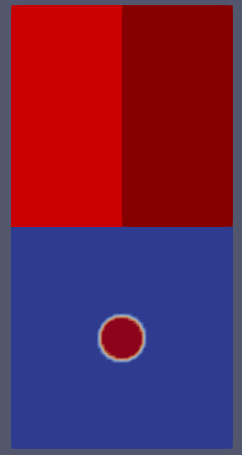
\includegraphics[scale=0.5]{../res/imgs/image8.png}
    \caption{\textbf{El problema elegido} En esta imagen se puede apreciar la geometría del problema elegido: dos líquidos immiscibles en un recipiente, y una burbuja en la parte inferior del mismo.}
\end{figure}

\begin{figure} 
    \centering
    
\includegraphics[scale=0.5]{../res/imgs/image5.png}
    \caption{\textbf{Subdivisión del problema }En esta figura se puede cómo se asigna un núcleo para cada parte de la figura.}
\end{figure}

\begin{figure} 
    \centering
    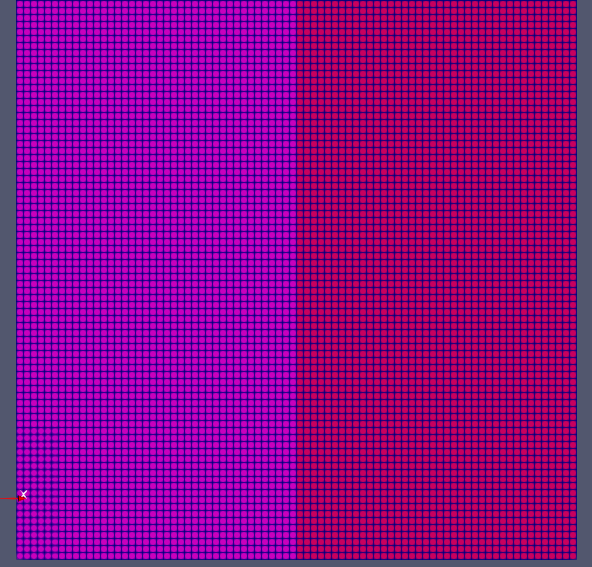
\includegraphics[scale=0.5]{../res/imgs/image3.png}
    \caption{\textbf{Detalle de la discretización} En esta imagen se ve en detalle la discretización, cómo cada core se subdivide en 3200 celdas (eje $y$ dividido en 40, el $x$ en 30). Notar que para realizar las operaciones en el límite de las caras se necesita información de varios procesadores distintos: es importante no pasar por alto este detalle, ya que es la variable que juega en contra de la paralelización por traer consigo un costo comunicacional extra. En el hipotético caso de tener 3200 cores para resolver este problema, claramente la situación no escala, debido a que el costo comunicacional terminaría ocupando la mayor porción del tiempo.}
\end{figure}

\begin{figure} 
    \centering
    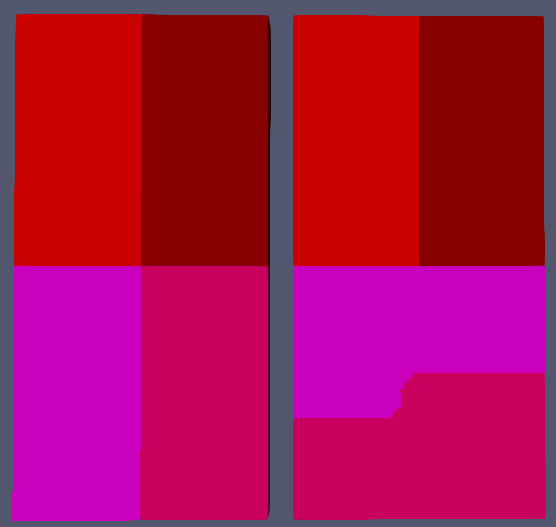
\includegraphics[scale=0.5]{../res/imgs/image6.png}
    \caption{\textbf{Descomposición Jerárquica vs. Scotch} En esta descomposición se puede ver que existe una ligera modificación en cómo se asignan las caras y la distribución de celdas en cada uno de los cores. Este tipo de descomposición es ideal para usar cuando la geometría del problema no es simétrica como en el caso del ejemplo, donde le trata de asignar a cada core la misma cantidad de celdas y minimizar las caras entre estos en base a un algoritmo u estrategia.}
\end{figure}

\newpage
\section{Ejecución}
\subsection{Monocore}
Para ejecutar el solver sin paralelismo, es suficiente con correr el comando \texttt{./Allrun}. El mismo se encarga de crear la malla de discretización y de correr el solver.
\subsection{Multicore}
Para la resolución con paralelismo se hace uso del MPI (Message Passing Interface) mediante el comando mpirun. Al mismo se le pasan flags indicando cantidad de procesadores y tipo de binding, tema que se cubrirá a continuación. Por un tema de prolijidad se sugiere redireccionar la salida del programa a un archivo log.

\begin{lstlisting}[caption={Ejemplo de comando a ejecutar para resolver con paralelismo.}, captionpos=b]
mpirun -np 4  compressibleInterFoam -parallel > log.6626
\end{lstlisting}

Al estar ejecutándose la simulación se puede ver el uso de cpu mediante comandos como \texttt{top} o \texttt{htop}: de acuerdo a la cantidad de procesadores que se haya decidido utilizar, se observa un uso cercano o igual al 100\% en las cpus en uso.
\begin{figure}[h!]
    \centering
    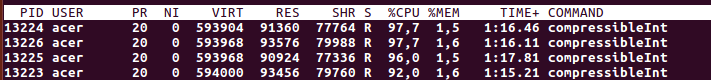
\includegraphics[scale=0.6]{../res/imgs/image7.png}
    \caption{Detalle de ejecución de \texttt{top}} 
\end{figure}
\subsubsection{Bindings}
El binding se setea mediante el flag --bind-to. Por defecto se hace --bind-to core, lo que asegura que un mismo proceso se corra siempre en el mismo procesador. Esto es positivo, ya que si el proceso se va cambiando de procesador, se pierde toda la información que el procesador haya guardado en sus registros o cache. Para desactivar esto, se usa --bind-to none.

El flag --bycore asegura que procesos secuenciales de MPI corran en procesadores adyacentes.

Lo esperado es que el binding incremente la performance, previniendo al sistema operativo mover procesos de un core a otro con el fin de balancear la carga.

\newpage
\section{Análisis de las ejecuciones}
En esta sección se realizará un análisis basado en gráficos que permitan apreciar los distintos speedups obtenidos con las distintas configuraciones.

Para el análisis se usará el tiempo real, ya que si bien contempla también tiempos no usados exclusivamente para el procesamiento, se la considera una medida más real debido al tiempo que se usa para comunicación. 

Los speedup fueron calculados tomando como tiempo viejo el tiempo necesario para correr el solver en un único núcleo, ya que es el único caso que no hace uso del paralelismo y se quiere ver cómo se puede mejorar a partir de ese caso paralelizando el problema.

\subsection{PC \#2}
\begin{figure}[h!]
    \includesvg[svgpath=../res/imgs/]{pc2cores2a4}
    \caption{Speedups de PC 2: cantidad de núcleos entre 2 y 4.}
\end{figure}
En esta PC se puede observar que ya usando dos núcleos se obtiene un speedup de 53\% en el mejor de los casos. Este speedup que supera el 50\% es muy bueno considerando que duplicando la cantidad de núcleos el óptimo teórico tiene un tope de 100\%, el cual se sabe que es inalcanzable en la práctica. Notar de todas formas que hay un 14\% de diferencia con el speedup obtenido en el peor caso. Si bien un speedup de 39\% es de todas formas muy bueno, es evidente ya desde el principio que los distintos tipos de binding juegan un papel clave en el manejo de la paralelización. 

En el caso de la corrida con 3 núcleos se observa que el mejor speedup fue alcanzado por dos de las tres técnicas de binding, logrando un speedup de 73\%. En este caso la diferencia con el peor speedup logrado es mucho menor, de tan solo 9\%. Sigue siendo, de todas formas, una diferencia significativa. A diferencia del caso anterior, se observa que se logra un cuarto del speedup óptimo teórico (300\%).

Fue necesario ocupar 4 núcleos para alcanzar un speedup del 100\%. La relación entre el óptimo teórico y el mejor real es igual al caso anterior: se logra solamente un cuarto del máximo teórico (400\%). Además se puede ver nuevamente que el binding juega un papel no menor, ya que la diferencia entre mejor y peor caso utilizando 4 núcleos es del 27\%. 

Como la PC en análisis cuenta con 8 subprocesos pero solamente 4 núcleos, será interesante ver los resultados de las mediciones subsiguientes. ¿Seguirá aumentando el speedup, o fue el máximo posible ya alcanzado?

\begin{figure}[h!]
    \includesvg[svgpath=../res/imgs/]{pc2cores5a8}
    \caption{Speedups de PC 2: cantidad de núcleos entre 5 y 8.}
\end{figure}
A primera vista se puede ver que los speedups obtenidos son todos inferiores al mejor speedup obtenido con hasta 4 núcleos.

En los casos de 5 y 6 núcleos casi no hay diferencia entre los distintos tipos de binding, mientras que en el caso de 7 núcleos, dependiendo del tipo de binding se puede obtener hasta un 21% de diferencia. 

En el caso de los 5 núcleos se observa un speedup de entre el 76% y 82%. 

En el caso de los 6 núcleos el speedup fue menor: en el mejor caso se alcanzó el 67% (peor caso: 62%). 

Con 7 núcleos la variedad de resultados desorienta bastante: en el mejor de los casos, el speedup es casi igual al peor caso de los 5 núcleos (!).

……

De todas estas mediciones con 5 o más núcleos, se pueden rescatar las siguientes observaciones contraintuitivas: en primer lugar, el máximo speedup fue logrado con 5 núcleos, que es la menor cantidad de la muestra observada. Por otro lado, este speedup es muy similar al speedup obtenido con 3 núcleos, lo que significa que todos los speedups con 5 o más están muy por detrás del speedup obtenido con 4 núcleos.

\subsection{PC \#3}
\subsubsection{Descomposicion Jerarquica}
\begin{figure}[H]
    \includesvg[svgpath=../res/imgs/]{pc3Jerarquica}
    \caption{Speedups de PC 3 con descomposición jerárquica}
\end{figure}

Con esta pc se puede ver que utilizando la descomposición jerárquica, ya usando solamente 2 núcleos se obtiene un excelente speedup, un poco mejor al 80\%, que es el 80\% del óptimo teórico posible: llama la atención, ya que no es común acercarse tanto al óptimo teórico. Notar, de todas formas, que si bien con dos tipos de binding se obtienen excelentes resultados, al usar bind to none by core, el speedup es muchísimo menor: solamente es del 30\%, teniendo un 50\% de diferencia con los otros dos tipos de binding (!). Indudablemente no es un detalle menor.

Con 3 núcleos se observa un desempeño relativamente parejo entre los tres tipos de bindings, habiendo solamente un 7\% de diferencia entre los casos extremos. Sorprende un poco que el speedup no sólo no haya mejorado con respecto al caso de los dos núcleos, sino que ha empeorado alrededor del 10\%.

En el caso de los 4 núcleos, los resultados son un tanto variables: en el mejor de los casos se obtiene un speedup del 75\%, mientras que en el peor de los casos el speedup obtenido es de 46\%, lo que hace una diferencia de 30\% entre los extremos. Nuevamente se observa que el speedup no supera al del caso de los 2 núcleos, y además es bastante parecido al obtenido con 3 núcleos. 

Indudablemente, la descomposición jerárquica ha sorprendido un poco con los resultados obtenidos.

\subsubsection{Descomposición Scotch}
\begin{figure}[H]
    \includesvg[svgpath=../res/imgs/]{pc3Scotch}
    \caption{Speedups de PC 3 con descomposición scotch}
\end{figure}
En el caso de la descomposición scotch con dos núcleos se midió un speedup de entre 75\% y 80\%. Nuevamente, como se comentó en el caso de la descomposición jerárquica, dicho speedup es excelente considerando que el máximo teórico es del 100%. 

Lamentablemente el speedup no sigue creciendo a medida que se agregan más núcleos: viendo los gráficos de 3 y 4 núcleos se puede ver que en ninguno de los casos se alcanza, con ninguno de los tres bindings posibles, el peor de los speedups obtenidos con solamente 2 núcleos.

\subsubsection{Jerarquica vs Scotch}
\begin{figure}[H]
    \includesvg[svgpath=../res/imgs/]{pc3Scotch}
    \caption{Speedups de PC 3 con descomposición scotch}
\end{figure}
Si bien se pueden observar pequeñas diferencias que en los tres casos favorecen a la descomposición Jerárquica, estas diferencias no son mayores. De todas formas toda la evidencia indica que es mejor trabajar con descomposición Jerárquica.

\newpage
\section{Conclusiones}
A partir de las mediciones se puede ver que no siempre se cumple que al agregar más procesadores aumenta el speedup. Esto tiene que ver con cuestiones planteadas al principio del trabajo: el costo comunicacional consume tiempo, y si bien es subconscientemente subestimado debido a que el enfoque está en la parte computacional, termina siendo evidente que no es un tema menor. 

Si bien en la PC 2 se pudo observar un speedup creciente a medida que se iba aumentando la cantidad de núcleos reales, no sucedió lo mismo con la PC 3, donde si bien no se esperaban valores exagerados e irreales que se acerquen demasiado al speedup óptimo teórico, sí se esperaba que aumente por lo menos un poco al agregar más núcleos para el cómputo.

\newpage
\section{Anexo}
\subsection{Mediciones}
La hoja de datos con las mediciones junto a los gráficos correspondientes están disponibles para una mejor apreciación en este \href{https://docs.google.com/spreadsheets/d/e/2PACX-1vQOSLYH4y81OxVleLZk2YwzFhrl4-AzE2-IUF04Y9lkk0pP6SZe1VFkkFW7r9lDK-Qo8OkGUuwHFlOE/pubhtml}{link}\footnote{https://docs.google.com/spreadsheets/d/e/2PACX-1vQOSLYH4y81OxVleLZk2YwzFhrl4-AzE2-IUF04Y9lkk0pP6SZe1VFkkFW7r9lDK-Qo8OkGUuwHFlOE/pubhtml}. 
\subsection{Código del caso}
\lstinputlisting[caption={\texttt{0.orig/alpha.water}}, captionpos=b]{../res/depthCharge2d/0.orig/alpha.water}
\lstinputlisting[caption={\texttt{0.orig/p}}, captionpos=b]{../res/depthCharge2d/0.orig/p}
\lstinputlisting[caption={\texttt{0.orig/p\_rgh}}, captionpos=b]{../res/depthCharge2d/0.orig/p\_rgh}
\lstinputlisting[caption={\texttt{0.orig/T}}, captionpos=b]{../res/depthCharge2d/0.orig/T}
\lstinputlisting[caption={\texttt{0.orig/U}}, captionpos=b]{../res/depthCharge2d/0.orig/U}
\lstinputlisting[caption={\texttt{constant/g}}, captionpos=b]{../res/depthCharge2d/constant/g}
\lstinputlisting[caption={\texttt{constant/thermophysicalProperties}}, captionpos=b]{../res/depthCharge2d/constant/thermophysicalProperties}
\lstinputlisting[caption={\texttt{constant/thermophysicalProperties.air}}, captionpos=b]{../res/depthCharge2d/constant/thermophysicalProperties.air}
\lstinputlisting[caption={\texttt{constant/thermophysicalProperties.water}}, captionpos=b]{../res/depthCharge2d/constant/thermophysicalProperties.water}
\lstinputlisting[caption={\texttt{constant/turbulenceProperties}}, captionpos=b]{../res/depthCharge2d/constant/turbulenceProperties}
\lstinputlisting[caption={\texttt{system/blockMeshDict}}, captionpos=b]{../res/depthCharge2d/system/blockMeshDict}
\lstinputlisting[caption={\texttt{system/controlDict}}, captionpos=b]{../res/depthCharge2d/system/controlDict}
\lstinputlisting[caption={\texttt{system/decomposeParDict}}, captionpos=b]{../res/depthCharge2d/system/decomposeParDict}
\lstinputlisting[caption={\texttt{system/fvSchemes}}, captionpos=b]{../res/depthCharge2d/system/fvSchemes}
\lstinputlisting[caption={\texttt{system/fvSolution}}, captionpos=b]{../res/depthCharge2d/system/fvSolution}
\lstinputlisting[caption={\texttt{system/setFieldsDict}}, captionpos=b]{../res/depthCharge2d/system/setFieldsDict}
\lstinputlisting[caption={\texttt{Allrun}}, captionpos=b]{../res/depthCharge2d/Allrun}
\lstinputlisting[caption={\texttt{Allclean}}, captionpos=b]{../res/depthCharge2d/Allclean}

\newpage
\addcontentsline{toc}{section}{References}
\begin{thebibliography}{9} 
    \bibitem{} 
        Why would be sometimes running CFD in parallel processing with 600 CPUs is faster than 800 CPUs even though it has more processors?  

        \url{https://www.researchgate.net/post/Why_would_be_sometimes_running_CFD_in_parallel_processing_with_600_CPUs_is_faster_than_800_CPUs_even_though_it_has_more_processors2} 
    \bibitem{time} 
        What do 'real', 'user' and 'sys' mean in the output of time(1)?

        \url{https://stackoverflow.com/questions/556405/what-do-real-user-and-sys-mean-in-the-output-of-time1}
    \bibitem{} 
        William Gropp.
        Parallel compuring and domain decomposition.

        \url{http://ftp.mcs.anl.gov/pub/tech_reports/reports/P257.pdf}
    \bibitem{paraview}
        Para view: \url{https://www.paraview.org/}.
    \bibitem{}
        OpenFOAM: \url{https://www.openfoam.com/}.
    \bibitem{}
        MPI FAQ: General run-time tuning: \url{https://www.open-mpi.org/faq/?category=tuning#using-paffinity-v1.4}.
\end{thebibliography}
\end{document}
